% Comparison charts: OSNIP (paper) vs fastProve (this work)
% Compile: pdflatex osnip_vs_fastprove_compare.tex
\documentclass[11pt,a4paper]{article}
\usepackage[margin=1.6cm]{geometry}
\usepackage[T1]{fontenc}
\usepackage[utf8]{inputenc}
\usepackage{lmodern}
\usepackage{amsmath,booktabs,array,xcolor}
\usepackage{tikz}
\usepackage{pgfplots}
\pgfplotsset{compat=1.18}
\usepackage{caption}
\usepackage{hyperref}

\definecolor{Cosnip}{HTML}{F58518}
\definecolor{Cstruct}{HTML}{54A24B}
\definecolor{Cfull}{HTML}{E45756}
\definecolor{Cbad}{HTML}{B279A2}
\definecolor{Cgrid}{HTML}{E0E0E0}
\definecolor{Cnote}{HTML}{555555}

\title{\textbf{Utility / Accuracy-Loss Comparison}\\
\large OSNIP (paper) vs.\ fastProve (this work)\\
\normalsize Focus: Llama-3.2-3B-Instruct}
\author{fastProve evaluation suite}
\date{\today}

\begin{document}
\maketitle
\vspace{-1.0em}

\noindent
{\small\color{Cnote}
OSNIP numbers from Cao et al.\ (preprint, Tables~1--3).
fastProve numbers from \texttt{results/raw/llama\_compare\_large.json}
(1500 real-scenario prompts $\times$ 3 master keys, BF16, RTX 5090).
\textbf{Metrics differ by design} --- see captions.}

\vspace{0.8em}

%==============================================================================
\subsection*{Figure 1 --- PPL relative increase on Llama-3.2-3B-Instruct
(lower is better)}
%==============================================================================
\begin{center}
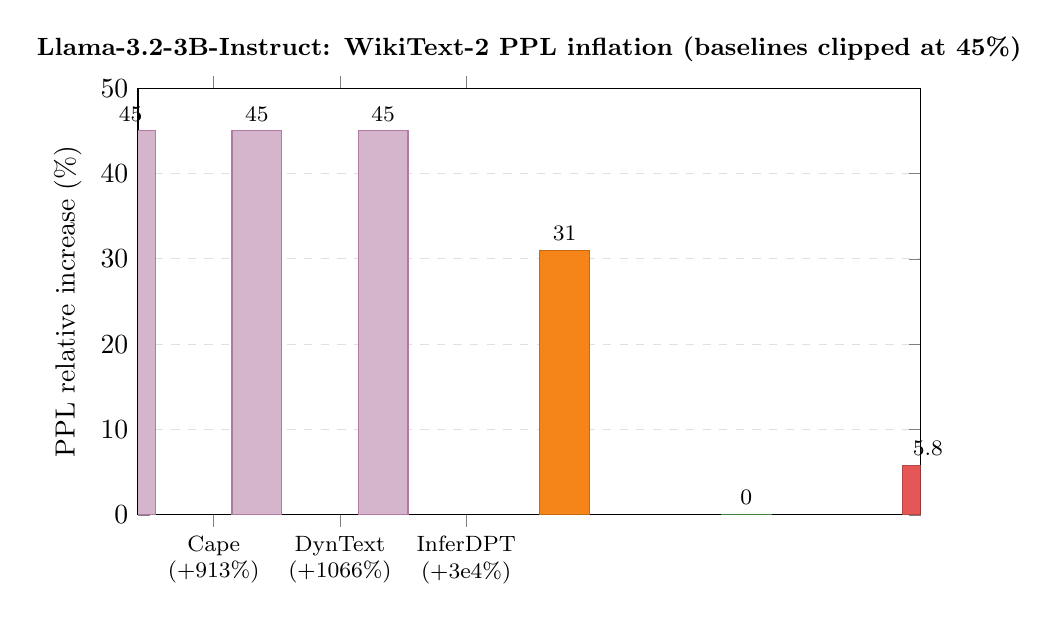
\begin{tikzpicture}
\begin{axis}[
  ybar,
  bar width=18pt,
  width=0.95\textwidth,
  height=7.0cm,
  ymin=0, ymax=50,
  ylabel={PPL relative increase (\%)},
  symbolic x coords={Cape,DynText,InferDPT,OSNIP,FPstruct,FPfull},
  xtick=data,
  xticklabels={{Cape\\(+913\%)},{DynText\\(+1066\%)},{InferDPT\\(+3e4\%)},{OSNIP\\(+31\%)},{FP struct\\($\approx$0\%)},{FP full\\(+5.8\%)}},
  xticklabel style={align=center, font=\footnotesize},
  enlarge x limits=0.12,
  nodes near coords,
  every node near coord/.append style={
    font=\footnotesize,
    /pgf/number format/fixed,
    /pgf/number format/precision=1,
  },
  ymajorgrids=true,
  grid style={Cgrid,dashed},
  title={Llama-3.2-3B-Instruct: WikiText-2 PPL inflation (baselines clipped at 45\%)},
  title style={font=\bfseries\small},
]
\addplot[fill=Cbad!55, draw=Cbad] coordinates {
  (Cape,45)
  (DynText,45)
  (InferDPT,45)
};
\addplot[fill=Cosnip, draw=Cosnip!80!black] coordinates {
  (OSNIP,31.0)
};
\addplot[fill=Cstruct, draw=Cstruct!80!black] coordinates {
  (FPstruct,0.02)
};
\addplot[fill=Cfull, draw=Cfull!80!black] coordinates {
  (FPfull,5.79)
};
\end{axis}
\end{tikzpicture}
\end{center}
{\footnotesize
True baseline $\Delta\%$ (OSNIP Table~2, same model):
Cape $+913\%$, DynText $+1066\%$, InferDPT $+29699\%$ (bars clipped).
OSNIP $+31\%$.
fastProve mean over 3 keys on 1500 prompts: structural $\approx 0\%$, full $+5.79\%$.
\\[0.25em]
\textbf{Takeaway:} On 3B PPL inflation, fastProve (struct./full) is \textbf{tighter than OSNIP}.
}

\vspace{0.9em}

%==============================================================================
\subsection*{Figure 2 --- Retention / fidelity (higher is better)}
%==============================================================================
\begin{center}
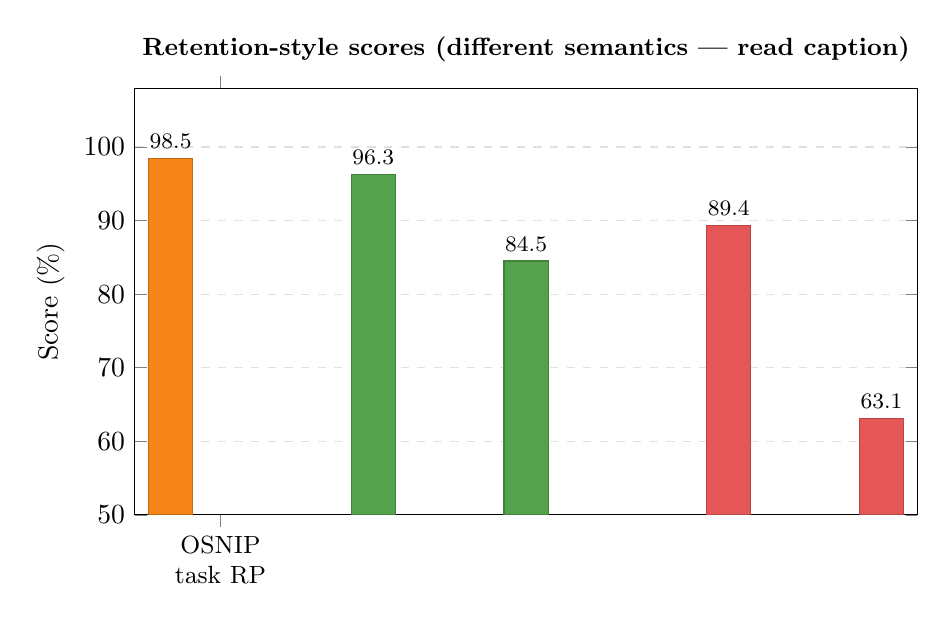
\begin{tikzpicture}
\begin{axis}[
  ybar,
  bar width=16pt,
  width=0.95\textwidth,
  height=7.0cm,
  ymin=50, ymax=108,
  ylabel={Score (\%)},
  symbolic x coords={OSNIPrp,FPtokS,FPgrdS,FPtokF,FPgrdF},
  xtick=data,
  xticklabels={{OSNIP\\task RP},{FP struct\\token},{FP struct\\greedy},{FP full\\token},{FP full\\greedy}},
  xticklabel style={align=center, font=\small},
  enlarge x limits=0.14,
  nodes near coords,
  nodes near coords style={
    font=\footnotesize,
    /pgf/number format/fixed,
    /pgf/number format/precision=1,
  },
  ymajorgrids=true,
  grid style={Cgrid,dashed},
  title={Retention-style scores (different semantics --- read caption)},
  title style={font=\bfseries\small},
]
\addplot[fill=Cosnip, draw=Cosnip!80!black] coordinates {
  (OSNIPrp, 98.49)
};
\addplot[fill=Cstruct, draw=Cstruct!80!black] coordinates {
  (FPtokS, 96.26)
  (FPgrdS, 84.51)
};
\addplot[fill=Cfull, draw=Cfull!80!black] coordinates {
  (FPtokF, 89.39)
  (FPgrdF, 63.13)
};
\end{axis}
\end{tikzpicture}
\end{center}
{\footnotesize
\textbf{OSNIP task RP:} average accuracy retained vs.\ non-private on 10 closed-ended
tasks (paper Table~1, Llama-3.2-3B-Instruct $=98.49\%$).
\textbf{FP token:} mean next-token top-1 agreement with plaintext path.
\textbf{FP greedy:} mean full generated-suffix exact match with plaintext
(1500 prompts $\times$ 3 keys).
\\[0.25em]
\textbf{Takeaway:} OSNIP reports near-lossless \emph{task} utility; fastProve reports \emph{trajectory} fidelity.
}

\vspace{0.9em}

%==============================================================================
\subsection*{Figure 3 --- Grouped multi-axis mapped scores}
%==============================================================================
\begin{center}
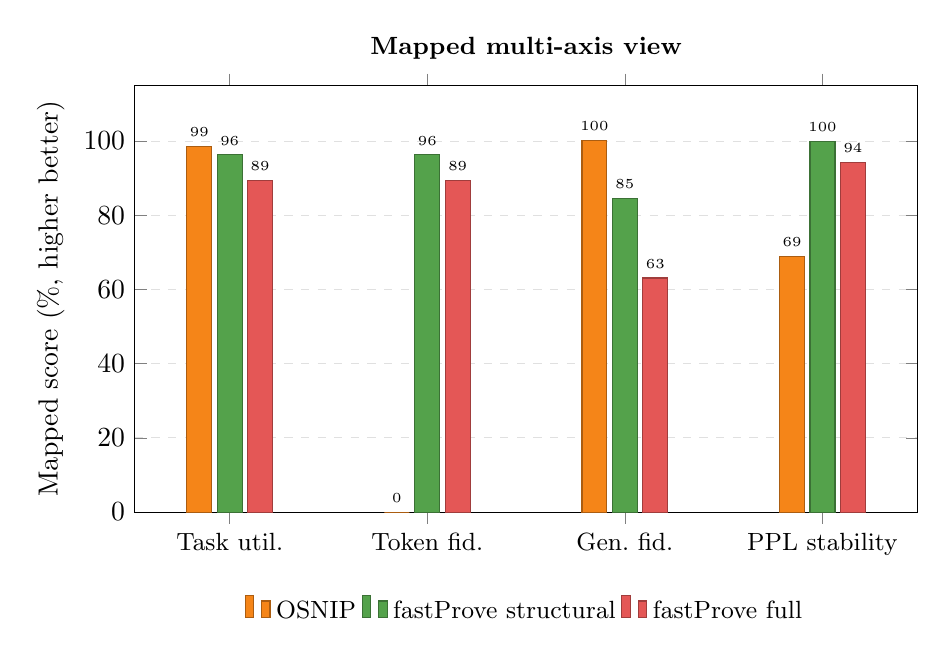
\begin{tikzpicture}
\begin{axis}[
  ybar,
  bar width=9pt,
  width=0.95\textwidth,
  height=7.0cm,
  ymin=0, ymax=115,
  enlarge x limits=0.16,
  legend style={
    at={(0.5,-0.18)},
    anchor=north,
    legend columns=3,
    font=\small,
    draw=none
  },
  ylabel={Mapped score (\%, higher better)},
  symbolic x coords={Task,Token,Gen,PPL},
  xtick=data,
  xticklabels={{Task util.},{Token fid.},{Gen.\ fid.},{PPL stability}},
  xticklabel style={font=\small},
  ymajorgrids,
  grid style={Cgrid,dashed},
  nodes near coords,
  every node near coord/.append style={
    font=\tiny,
    /pgf/number format/fixed,
    /pgf/number format/precision=0
  },
  title={Mapped multi-axis view},
  title style={font=\bfseries\small},
]
% OSNIP: task RP 98.5; token n/a=0; gen BERTScore RP 100.1; PPL stab 100-31=69
\addplot[fill=Cosnip, draw=Cosnip!70!black] coordinates {
  (Task, 98.5)
  (Token, 0)
  (Gen, 100.1)
  (PPL, 69)
};
% structural
\addplot[fill=Cstruct, draw=Cstruct!70!black] coordinates {
  (Task, 96.3)
  (Token, 96.3)
  (Gen, 84.5)
  (PPL, 100)
};
% full
\addplot[fill=Cfull, draw=Cfull!70!black] coordinates {
  (Task, 89.4)
  (Token, 89.4)
  (Gen, 63.1)
  (PPL, 94.2)
};
\legend{OSNIP, fastProve structural, fastProve full}
\end{axis}
\end{tikzpicture}
\end{center}
{\footnotesize
\textbf{Mapping:}
Task util.\ = OSNIP RP; fastProve bars use token agreement as a \emph{proxy only} (no MMLU yet).
Token fid.\ = OSNIP not reported (bar $0$ = n/a).
Gen.\ fid.\ = OSNIP BERTScore retention on CNN/DM (Table~3); fastProve greedy exact match.
PPL stability $= 100 - \Delta_{\mathrm{PPL}}\%$ (OSNIP $69$).
}

\vspace{0.7em}

%==============================================================================
\subsection*{Summary table}
%==============================================================================
\begin{center}
\small
\begin{tabular}{@{}lcccc@{}}
\toprule
\textbf{Method} &
\textbf{Task RP (\%)$\uparrow$} &
\textbf{Token agree (\%)$\uparrow$} &
\textbf{Greedy (\%)$\uparrow$} &
\textbf{PPL $\Delta\%$ $\downarrow$} \\
\midrule
Plaintext / non-private & 100 & 100 & 100 & 0 \\
OSNIP (paper, 3B) & \textbf{98.49} & --- & ---$^{\dagger}$ & $+31$ \\
Cape / DynText / InferDPT & 48--73 & --- & --- & $\gg 700$ \\
\addlinespace
fastProve structural & --- & \textbf{96.26} & 84.51 & \textbf{$\approx 0$} \\
fastProve full & --- & 89.39 & 63.13 & $+5.79$ \\
\bottomrule
\end{tabular}\\[0.3em]
{\footnotesize $^{\dagger}$OSNIP reports near-lossless summarization BERTScore RP ($\approx 100\%$), not greedy match to plaintext.}
\end{center}

\vspace{0.5em}
\subsection*{Bottom line}
\begin{enumerate}
  \item \textbf{PPL:} fastProve structural / full control inflation better than OSNIP on 3B
  ($0$ / $+6\%$ vs $+31\%$).
  \item \textbf{Task suite:} OSNIP has stronger published evidence of near-lossless accuracy
  retention; fastProve still needs the same MMLU-style suite for a fair win claim.
  \item \textbf{Trajectory:} only fastProve measures plaintext token/greedy agreement directly
  (struct.\ $\sim 96\%$/ $85\%$; full $\sim 89\%$/ $63\%$).
\end{enumerate}

\vspace{0.3em}
{\scriptsize\color{Cnote}
Sources: OSNIP Tables 1--3 (Llama-3.2-3B-Instruct);
fastProve \texttt{llama\_compare\_large.json} (mean over 3 keys).
}
\end{document}
